% % % % % % % % % % % % % % % % % % % % % % % % % % % % % % % % % % % % % % % % %
%
% LaTeX Presentation Template
%
% This template is based on Hannes Badertschers HSR presentation template
% See https://github.com/HBadertscher/HSRPresentation
% % % % % % % % % % % % % % % % % % % % % % % % % % % % % % % % % % % % % % % % %
% "THE BEER-WARE LICENSE" (Revision 42):
% Patrik Müller (p1muelle@hsr.ch) wrote this LaTeX template. As long as you retain
% this notice you can do whatever you want with this stuff. If we meet some day,
% and you think this stuff is worth it, you can buy me a beer in return.
% - Patrik Müller
% % % % % % % % % % % % % % % % % % % % % % % % % % % % % % % % % % % % % % % % %

\RequirePackage[l2tabu, orthodox]{nag}    % Warnings for obsolete packages
\RequirePackage{etex}                     % Load e-TeX engine
\documentclass[aspectratio=169,envcountsect]{beamer}    % 169 (16:9) or 43 (4:3)
\usepackage[utf8]{inputenc}               % Always use UTF-8!

\newcommand*{\Title}{Your Presentation Title}
\newcommand*{\TitleShort}{Short Version of the Title}
\newcommand*{\Subtitle}{Your fancy Subtitle}
\newcommand*{\Author}{Your Name}
\newcommand*{\AuthorShort}{Y. Name}
\newcommand*{\Topic}{Topic}
\newcommand*{\Lang}{en}
%\newcommand*{\Institute}{institutes/ICOM-Institute_for_Communication_System_CMYK.eps}
\newcommand*{\Institute}{Institute / Department}
\newcommand*{\InstituteShort}{Inst}
\newcommand*{\TitlepageType}{1}
\newcommand*{\Location}{rapperswil}
\newcommand*{\TocAtSection}{true}
\newcommand*{\TocSplit}{9}
\newcommand*{\SubtitleInHeader}{true}
\newcommand*{\ProgressBar}{false}

\usepackage{xstring}
\usepackage{setspace}
\newcommand{\OstToc}[1][]{
	\IfInteger{\TocSplit}
	{
		\tikzmath{integer \nextsection; \nextsection = \TocSplit+1;}
		\begin{columns}[t]
			\begin{column}{0.5\textwidth}
				\tableofcontents[sections=1-\TocSplit, #1]
			\end{column}
			\begin{column}{0.49\textwidth}
				\tableofcontents[sections=\nextsection-, #1]
			\end{column}
		\end{columns}
	}
	{\tableofcontents}
}

% % % % % % % % % % % % % % % % % % % % % % % % % % % % % % % % % % % % % % % % %
%
% LaTeX Presentation Template - Header File
%
% % % % % % % % % % % % % % % % % % % % % % % % % % % % % % % % % % % % % % % % %
% "THE BEER-WARE LICENSE" (Revision 42):
% Patrik Müller (p1muelle@hsr.ch) wrote this LaTeX template. As long as you retain 
% this notice you can do whatever you want with this stuff. If we meet some day, 
% and you think this stuff is worth it, you can buy me a beer in return. 
% - Patrik Müller
% % % % % % % % % % % % % % % % % % % % % % % % % % % % % % % % % % % % % % % % %

% Packages
\usetheme{default}

% Fonts
\usepackage[T1]{fontenc}
\usepackage[sc]{mathpazo}               % use palatino font!
\linespread{1.05}                       % palatino needs a bit more space!
\usepackage[T1,small,euler-digits]{eulervm}
\usepackage[scaled=0.8]{beramono}       % Use bera for mono fonts
\usefonttheme{professionalfonts}        % Setup beamer to use these fonts

% Math
\usepackage{amsmath}
\usepackage{amssymb}

% Babel
\newcommand*{\LangDE}{de}
\ifx \Lang \LangDE
    \usepackage[english,ngerman]{babel}
\else
    \usepackage[ngerman,english]{babel}
\fi

% Tables
\usepackage{booktabs}
\usepackage{tabularx}
\usepackage{multicol}

% Colors
\usepackage{xcolor}
\usepackage{header/ost_colors}

% Graphics
\usepackage{graphicx}
\usepackage{caption}
\usepackage{epstopdf}
\usepackage{tikz}
\usetikzlibrary{arrows,backgrounds,fit,positioning,calc,shapes}
\usepackage[american currents]{circuitikz}
\usepackage{tikz-timing}[2009/12/09]
\usepackage{pgfplots}
\pgfplotsset{compat = 1.3}

% Listings
\usepackage{listings}

% SI Units
\usepackage{siunitx}
\sisetup{detect-all,sticky-per,per-mode=symbol}

% Chemical formulae
\usepackage[version=3]{mhchem}

% EToolbox for e-TeX (programming)
\usepackage{etoolbox}

% HSR Colorbox
\usepackage{tcolorbox}
\newtcolorbox{ostbox}[1]{colback=OSTwhite,colframe=OSTblackberry,title=#1}

% Setup date-time format
\usepackage{datetime}
\newdateformat{titledate}{\THEDAY.~\monthname\space\THEYEAR}

\newcommand*{\TypeBubble}{bubble}
\newcommand*{\Background}{backgrounds/title_\Location_\TitlepageType}
\setbeamertemplate{navigation symbols}{}

% % % % % % % % % % % % % % % % % % % % % % % % % % % % % % % % % % % % % % % % %
% Setup Document
\title[\TitleShort]{\Title}
\subtitle{\Subtitle}
\author[\AuthorShort]{\Author}

\hypersetup{
    pdftitle={\Title},
    pdfauthor={\Author},
    pdfsubject={\Subtitle},
    pdfcreator={LaTeX with hyperref and Beamer}
}

% % % % % % % % % % % % % % % % % % % % % % % % % % % % % % % % % % % % % % % % %
% Color scheme
\setbeamercolor*{frametitle}{fg=white,bg=OSTblackberry}
\setbeamertemplate{section in toc}{\hspace{1em}{\scriptsize\color{OSTblackberry}$\blacksquare$}~\inserttocsection}
\setbeamercolor*{section in toc}{fg=OSTblack}
\setbeamercolor*{section in toc shaded}{fg=OSTblack}

\setbeamertemplate{itemize item}[circle]
\setbeamercolor*{itemize item}{fg=OSTblackberry}
\setbeamertemplate{itemize subitem}[circle]
\setbeamercolor*{itemize subitem}{fg=OSTlightgray}
\setbeamertemplate{itemize subsubitem}[triangle]
\setbeamercolor*{itemize subsubitem}{fg=OSTlightgray}

\setbeamertemplate{enumerate item}{\arabic{enumi})}
\setbeamercolor{enumerate item}{fg=OSTblackberry}
\setbeamertemplate{enumerate subitem}{\roman{enumii})}
\setbeamercolor{enumerate subitem}{fg=black}
\setbeamertemplate{enumerate subsubitem}{\alph{enumiii})}
\setbeamercolor{enumerate subsubitem}{fg=black}

\setbeamertemplate{caption}{\scshape\scriptsize\textcolor{OSTblackberry}{\insertcaptionname:}~\insertcaption}


% % % % % % % % % % % % % % % % % % % % % % % % % % % % % % % % % % % % % % % % %
% Title page
\defbeamertemplate*{title page}{customized}[1][]{
    \begin{tikzpicture}[remember picture,overlay,shift=(current page.south west)]

        \useasboundingbox (0,0) rectangle (\the\paperwidth,\the\paperheight);

        % Background image
%        \node at (current page.center) {\includegraphics[width=\the\paperwidth]{\Background}};

		\ifx \TitlepageType \TypeBubble
			 % Text
			\node[anchor=north west] at (63.4mm, 10.1mm) (institute){\parbox{80mm}{\scriptsize\Institute}};
			\node[anchor=south west, above=1.5mm of institute] (date) {\parbox{80mm}{\scriptsize\titledate\today}};
			\node[anchor=south west, above=0mm of date] (author) {\parbox{80mm}{\scriptsize\Author}};
			\node[inner ysep=0, outer sep=0, above=1.2cm of author.north west, anchor=north west] (subtitle) {\parbox{80mm}{\textbf{\color{OSTblack}\large\Subtitle}}};
			\node[anchor=south west, inner ysep=0, outer sep=0, text height=1cm, above=2mm of subtitle] (title) {\parbox{80mm}{\textbf{\color{OSTblackberry}\LARGE\Title}}};
		\else
			% OST bars
			\draw[draw=none,fill=OSTblackberry,opacity=0.85] (6.8mm,9.1mm) rectangle (86.8mm,89.1mm);
			
			% OST logo
%			\draw[draw=none,fill=white] (0mm,4.5mm) rectangle (34.5mm,16.4mm);
%			\node[anchor=south west,inner sep=0] at (4.5mm,4.5mm) {
\includegraphics[width=30mm]{header/ost_logo}};
		\fi
    \end{tikzpicture}
}

% % % % % % % % % % % % % % % % % % % % % % % % % % % % % % % % % % % % % % % % %
% Footer
\newcommand*{\True}{true}
\setbeamertemplate{footline}
{
    \begin{tikzpicture}
        \pgfmathparse{\paperwidth/\inserttotalframenumber*\insertframenumber}
        \pgfmathresult \let\hsrBeamerProgressWidth\pgfmathresult

        \useasboundingbox (0,0) rectangle (\the\paperwidth,1.2cm);
        \draw[color=OSTblack] (0,1.2cm) -- (\the\paperwidth,1.2cm);

        \ifx \ProgressBar \True
            \draw[draw,fill] (0,1.2cm) rectangle (\hsrBeamerProgressWidth pt,1.15cm);
        \fi

        \node[inner sep=0pt,anchor=west] at (1em,0.6cm)  {
\includegraphics[width=2.5cm]{header/ost_logo}};

        \node[inner sep=0pt,anchor=center] at (0.5*\the\paperwidth,0.8cm){\scriptsize{\insertframenumber}};
        \node[inner sep=0pt,anchor=center] at (0.5*\the\paperwidth,0.4cm){\scriptsize{\AuthorShort}};

        \ifdefempty{\Institute}{}{
            \node[inner sep=0pt,anchor=east] at (\the\paperwidth-1em,0.6cm) {\InstituteShort};
        }

    \end{tikzpicture}
}

% % % % % % % % % % % % % % % % % % % % % % % % % % % % % % % % % % % % % % % % %
% TOC at beginning of every section

\ifx \TocAtSection \True
    \AtBeginSection[]
    {
        \begin{frame}<beamer>
            \frametitle{\contentsname}
            \tableofcontents[currentsection]
        \end{frame}
    }
\fi

\makeatletter
\patchcmd{\beamer@sectionintoc}{\vfill}{\vskip 8pt}{}{}
\makeatother
% % % % % % % % % % % % % % % % % % % % % % % % % % % % % % % % % % % % % % % % %
\begin{document}

\frame[plain]{\titlepage}

\section*{\contentsname}
\begin{frame}
 \OstToc{}
\end{frame}

\section{Lists}
\subsection{Unordered Lists}
\begin{frame}{Itemize}
 \begin{itemize}
  \item This is a ordered list
        \begin{itemize}
         \item Oh,
         \item So they can also be nested?
               \begin{itemize}
                \item One more for good measure
                \item What an amazing tool
               \end{itemize}
         \item Pretty nice, right?
        \end{itemize}
  \item Have fun!
 \end{itemize}
\end{frame}

\subsection{Ordered Lists}
\begin{frame}{Enumerate}
 The Data Science Skills that will get you hired
 \begin{enumerate}
  \item Programming Skills
        \begin{enumerate}
         \item Python
               \begin{enumerate}
                \item Numpy
                \item Pandas
                \item Matplotlib
               \end{enumerate}
         \item SQL
        \end{enumerate}
  \item Statistics
  \item Machine Learning
  \item Data Wrangling
  \item Data Visualization \& Communication
  \item Software Engineering
 \end{enumerate}
\end{frame}

\section{Math}
\begin{frame}{Equations}
 \begin{itemize}
  \item Here's an equation for you
        \[
         \iiint_V \left( \nabla \cdot \vec{F} \right) dV = \oiint_{\partial V} \vec{F}\cdot d\vec{S}
        \]
  \item Using \texttt{align}
        \begin{align}
         X[k] = \sum_{n=0}^{L-1}x[n]e^{-j\frac{2\pi}{N}n}
        \end{align}
  \item Some inline math \(\alpha=1-\sqrt{x^2+y^2}, \Delta\theta_i=(\theta-\theta_i)\mod 2\pi, \theta=\text{atan2}(y,x)\)
 \end{itemize}
\end{frame}

\section{Blocks \& Boxes}
\subsection{Text Blocks}
\begin{frame}{Block}
 \begin{block}{}
  Block without a title
 \end{block}
 \begin{block}{A block}
  Normal block with a title
 \end{block}
 \begin{alertblock}{Alert Block}
  Alerting content
 \end{alertblock}
 \begin{exampleblock}{Example Block}
  Example content
 \end{exampleblock}
\end{frame}

\subsection{Math Boxes}
\begin{frame}{Theorems}
 \begin{theorem}[Central Limit Theorem]
  Let \(X_{i}\), with \(1 \leq i \leq n\), be a sequence of mutually independent random variables with a common distribution \(X\). Suppose that \(\mu = E[X]\) and \(\varsigma^2=\text{Var}[X]\) exist and let \(S_n = \sum_{i=1}^n X_i\). Then, for every fixed \(\beta \)
  \[
   \lim_{n\to\infty} P\left[\frac{S_n - n\mu}{\varsigma\sqrt{n}} < \beta \right] = \Phi(\beta)
  \]
 \end{theorem}
\end{frame}

\begin{frame}{Definition}
 \begin{definition}[Feistel Cipher]
  A Feistel cipher is an iterated cipher mapping a \(n = 2t\) bits plain-text (which we denote \((L_0,R_0)\)), for \(t\)-bits blocks \(L_0\) and \(R_0\), to a cipher-text \((R_r,L_r)\), through a \(r\)-round process, where \(r\geq 1\). For \(1 \leq i \leq r\), round \(i\) maps \((L_{i-1},R_{i-1}) \underset{K_i}{\rightarrow} (L_i,R_i)\) as follows:
  \[
   \left\{\begin{array}{l}
    L_i = R_{i-1} \\
    R_i = L_{i-1} \oplus f(R_{i-1},K_i)
   \end{array}\right.
  \]
 \end{definition}
\end{frame}

\subsection{Quotation}
\begin{frame}{Quotes}
 \begin{quote}{}
  I'm an anonymous quote.
 \end{quote}
 \begin{quote}{Winston Churchill}
  A lady came up to me one day and said `Sir! You are drunk', to which I replied `I am drunk today madam, and tomorrow I shall be sober but you will still be ugly.
 \end{quote}
\end{frame}

\section{Figures and Tables}
\begin{frame}{Figure}
 \begin{figure}[h]
  \centering
  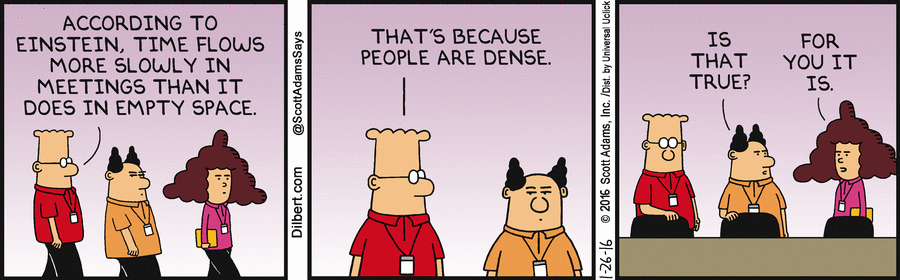
\includegraphics[width=.8\textwidth]{images/example}
  \caption{Example figure}
  \label{fig:ex1}
 \end{figure}
\end{frame}

\begin{frame}{tikz-Graphic}
 \begin{figure}[h]
  \centering
  \scalebox{0.7}{
\begin{tikzpicture}[myarrow/.style={->,>={Stealth[inset=0pt,length=8pt,angle'=60,round]}}]
	\draw
		(0,0) node(start){}
		(start) node[left]{AF signal}
		(3,-2.5) node[twoportshape,t=$90^\circ$,anchor=east](shift1){}
		(4.5,2.5) node[mixer](mix1){}
		(mix1.north) node[above]{Mixer}
		(4.5,-2.5) node[mixer](mix2){}
		(mix2.south) node[below]{Mixer}
		(8,0) node[adder](add){}
		(10,0) node[ampshape](pa){}
		(12,0) node[antenna](ant){}
		(ant) node[above=2.1cm]{Tx}
		(pa.north) node[above]{PA}
		(start) to (1,0)
		(1,0) |- (shift1.west)
		(add.east) to (pa.west)
		(pa.east) -- (ant);
	\draw[myarrow](1,0) |- (mix1.in);
	\draw[myarrow](shift1.east) -- (mix2.in);
	\draw[myarrow](mix1.out)-|node[pos=0.95,xshift=0.4cm]{\Large +}(add.north);
	\draw[myarrow](mix2.out)-|node[pos=0.95,xshift=0.4cm]{\Large +}(add.south);
	\draw 
		(3,0.5) node[oscillator](lo){}
		(lo.south) node[below]{LO}
		(4.5,-0.75) node[twoportshape,t=$90^\circ$](shift2){}
		(lo.east)-|(shift2.north);
	\draw[myarrow](lo.east)-|(mix1.south);
	\draw[myarrow](shift2.south)--(mix2.north);
	%(0,0) node[spdt] (Sw) {}
	%(Sw.in) node[left] {in}
	%(Sw.out 1) node[right] {out 1}
	%(Sw.out 2) node[right] {out 2};
\end{tikzpicture}}

  \caption{SSB Tx with Phasing Method}
  \label{fig:ex2}
 \end{figure}
\end{frame}

\begin{frame}{Table}
 \begin{table}[h]
  \centering
  \caption{Tic-Tac-Toe}\label{tab:tictactoe}
  {\Large
   \begin{tabular}{c|c|c}
    % \toprule
    x & o & x \\\midrule
    o & x & o \\\midrule
    o & x & x \\
		% \bottomrule
   \end{tabular}}
 \end{table}
\end{frame}

\section{Columns}
\begin{frame}{Columns and graphics}
	\begin{columns}[onlytextwidth]
  	\begin{column}{0.5\textwidth}
   		\begin{itemize}
    		\item Multi-col environments should be made using \texttt{columns}!
    		\item \emph{Never} use \texttt{minipage}'s or \texttt{multicols}.
   		\end{itemize}
  	\end{column}
  \begin{column}{0.5\textwidth}
  	\centering
   	
\includegraphics[width=0.6\linewidth]{header/ost_logo}
   	\captionof{figure}{A sample image. You don't need any floats here, just
    use \texttt{captionof}.}
  \end{column}
 \end{columns}
\end{frame}
%

\section*{}
\begin{frame}{The End}
 \begin{center}
  \def\s{4.8}
  \begin{tikzpicture}[state/.style={circle,minimum width=1.4cm,font=\scriptsize,fill=OSTlightpurple,draw},
    event/.style={->, -latex, font=\tiny}]
   % Draw state nodes
   \node[state] at (\s/2, {sqrt(3)/2*\s}) (busy) {Busy};
   \node[state] at (\s/2, {sqrt(3)/6*\s}) (normal) {Normal};
   \node[state] at (0, 0) (sleep) {Sleeping};
   \node[state] at (\s, 0) (hungry) {Hungry};

   % Draw event arrows
   \draw[event] (sleep) to node[midway,above,sloped] {get up}(normal);
   \draw[event] (normal) to node[midway,above,sloped] {study}(busy);
   \draw[event] (hungry) to node[midway,above,sloped] {eat}(normal);
   \draw[event] (busy) to [bend right=45] node[midway,above,sloped]{get tired} (sleep);
   \draw[event] (sleep) to [bend right=45] node[midway,above,sloped]{get hungry} (hungry);
   \draw[event] (busy) to [bend left=45] node[midway,above,sloped]{get hungry} (hungry);
  \end{tikzpicture}
 \end{center}
 %    \centering
 %    \LARGE That's all folks!
\end{frame}

\end{document}
% % % % % % % % % % % % % % % % % % % % % % % % % % % % % % % % % % % % % % % % %
